\begin{pastexam}[label={px:ncku-114-cce-ds-02}]{成大電通所 114 學年度 單選題第 2 題}
（單選；每題 5 分，答錯倒扣 2 分）

Given that the post-order traversal of a binary tree is ``E F B C D A'' and the in-order traversal of the same
tree is ``E F A C B D'', please provide the resulting pre-order traversal of the tree.
\begin{enumerate}[label=\alph*),nosep]
\item A F E D C B
\item A E F D C B
\item A F E C D B
\item A F E B C D
\item None of the above.
\end{enumerate}
\end{pastexam}

\begin{pastsoln}
答案：a) A F E D C B。

後序加中序決定唯一的二元樹（資結書第~7.4~節）：後序的最後一個是根，在中序裡找到根，左邊是左子樹、右邊是右子樹；
左子樹有幾個節點，後序的前面就取幾個給左子樹。
\begin{center}
\begin{tabular}{llcll}
\toprule
子樹的後序 & 子樹的中序 & 根 & 左子樹 & 右子樹 \\
\midrule
E F B C D A & E F $\mid$ A $\mid$ C B D & A & 中序 E F、後序 E F & 中序 C B D、後序 B C D \\
E F & E $\mid$ F $\mid$ & F & E & 空 \\
B C D & C B $\mid$ D $\mid$ & D & 中序 C B、後序 B C & 空 \\
B C & $\mid$ C $\mid$ B & C & 空 & B \\
\bottomrule
\end{tabular}
\end{center}
樹是：A 的左子節點 F、右子節點 D；F 的左子節點 E；D 的左子節點 C；C 的右子節點 B。
\begin{center}
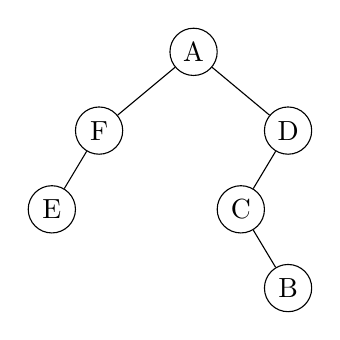
\begin{tikzpicture}[v/.style={circle,draw,inner sep=1pt,minimum size=6mm},
  level distance=10mm, level 1/.style={sibling distance=24mm}, level 2/.style={sibling distance=12mm}]
\node[v] {A}
  child {node[v] {F} child {node[v] {E}} child[missing] {}}
  child {node[v] {D} child {node[v] {C} child[missing] {} child {node[v] {B}}} child[missing] {}};
\end{tikzpicture}
\end{center}
前序（根、左、右）：A，左子樹 F E，右子樹 D C B，得 A F E D C B，選 a)。 檢查：這棵樹的後序是 E F B C D A、中序是
E F A C B D，和題目相符。 其他選項都和這個不同：b) 把 E、F 的上下顛倒；c)、d) 的右子樹部分順序錯。
\end{pastsoln}
